\subsection{Findings}
\label{sec:anal_findings}

Our first finding defends our first claim that there will be greater reward and punishment in our new solution than our previous prediction-based solution. We can determine a greater level of reward and punishment by looking at the percentage of transactions that were elevated due to a conflict. Our formula for calculating the percentage of elevated transactions is below:

\[\textrm{$T_{elevate}$} = \textrm{\# of executions that caused an ELEVATE}\]
\[\textrm{$T_{total}$} = \textrm{Total \# of executions}\]
\[\textrm{$P_{reward}$} =\frac{\textrm{$T_{elevate}$}}{\textrm{$T_{total}$}} \times 100\]
 
After analyzing the results we discovered that the $P_{reward}$ for the dynamic reputation solution is 51.9\% and the $P_{reward}$ for the prediction-based solution is 7.1\%. This is expected given that the reputation management solution involves a much more granular approach to establishing dominance that the four category system in the previous prediction-based solution. Therefore, this confirms that the dynamic reputation solution allows for a greater percentage of reward and punishment among the conflicting transactions.

Our second finding defends our second claim that we will see the reward and punishment reflected in the rankings of the users and transactions. By seeing a variance in the rankings of the users and transactions (see Definitions \ref{def:commit_ranking}, \ref{def:efficiency_ranking}, \ref{def:user_ranking},  and \ref{def:system_abort_ranking}) then we can confirm that our recalculations are causing changes in dominance based on the reputations of users and transactions. Figure \ref{image:variance_of_transaction_rankings} and \ref{image:variance_of_user_rankings} are two graphs showing the variance in the growth/reduction of transaction and user rankings across executions. You can see the rankings shrinking and growing as recalculations occur. Figure \ref{image:variance_of_transaction_rankings} shows the transaction rankings changing throughout the system. The y-axis represents the variance. The x-axis is the transaction ID (not shown for view ability). This graph represents all transactions that executed more than once within the system in order to show the changes in rankings between executions.

Figure \ref{image:variance_of_user_rankings} shows the same variance but for user rankings as they change throughout the system due to recalculation. The graph shows that the reward and punishment is actively being applied throughout the system.

\begin{figure}
\centering
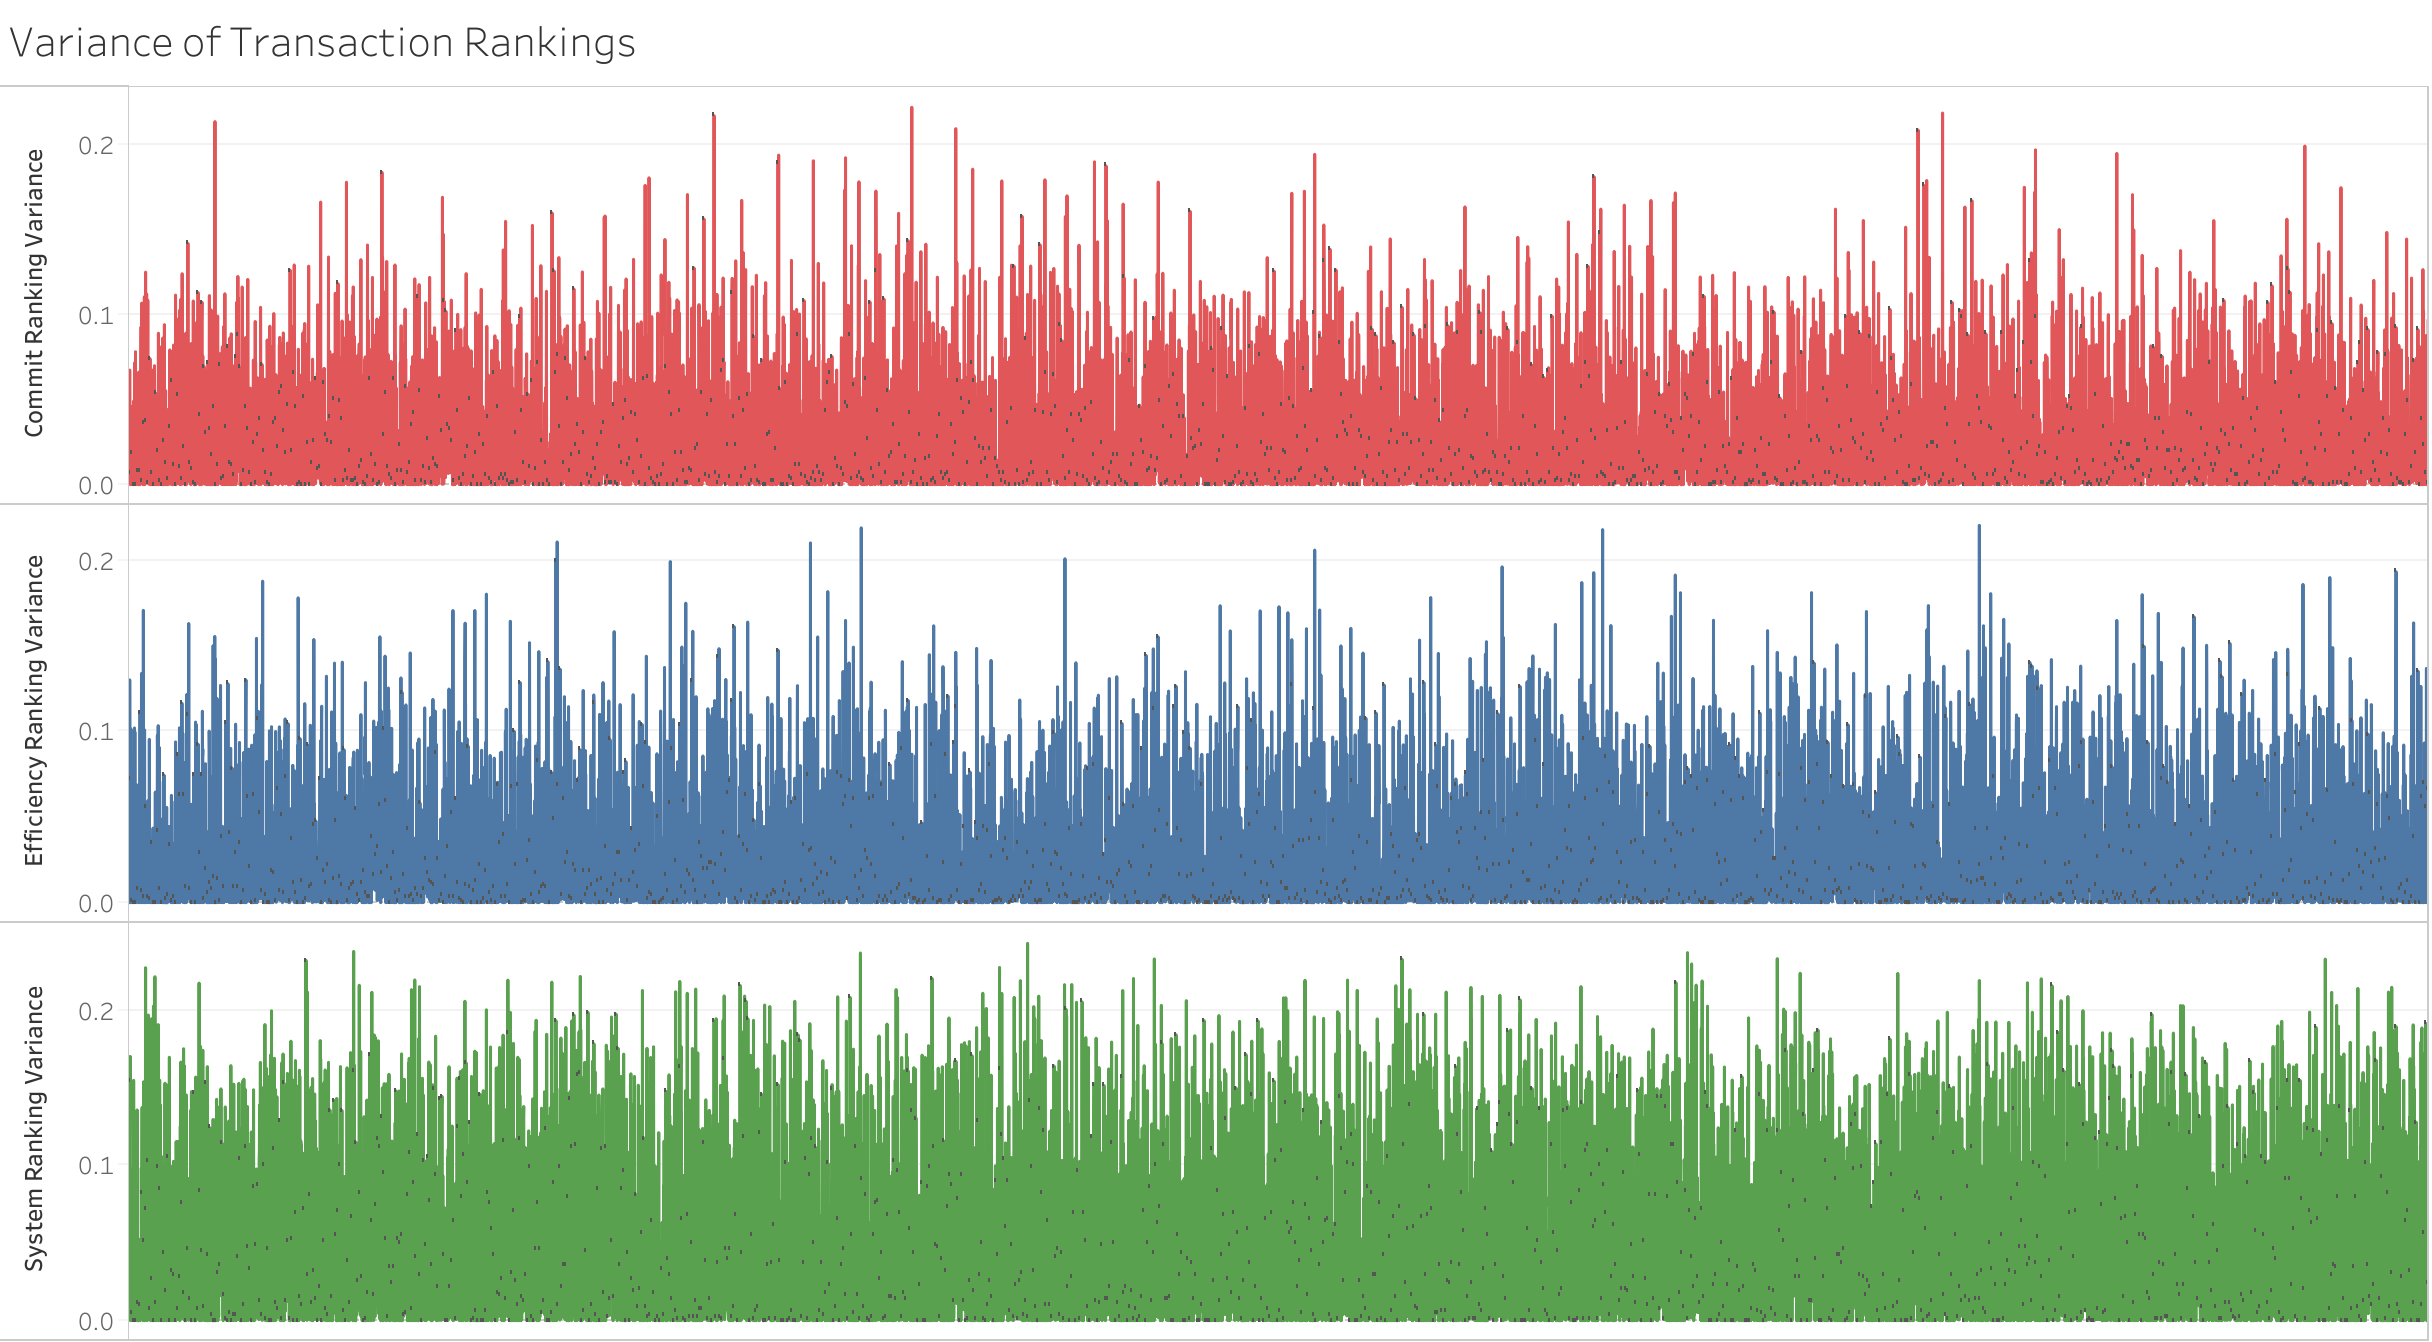
\includegraphics[scale=0.20]{images/VarianceofTransactionRankings.png}
\caption{Variance of Transaction Rankings}
\label{image:variance_of_transaction_rankings}
\end{figure}

\begin{figure}
\centering
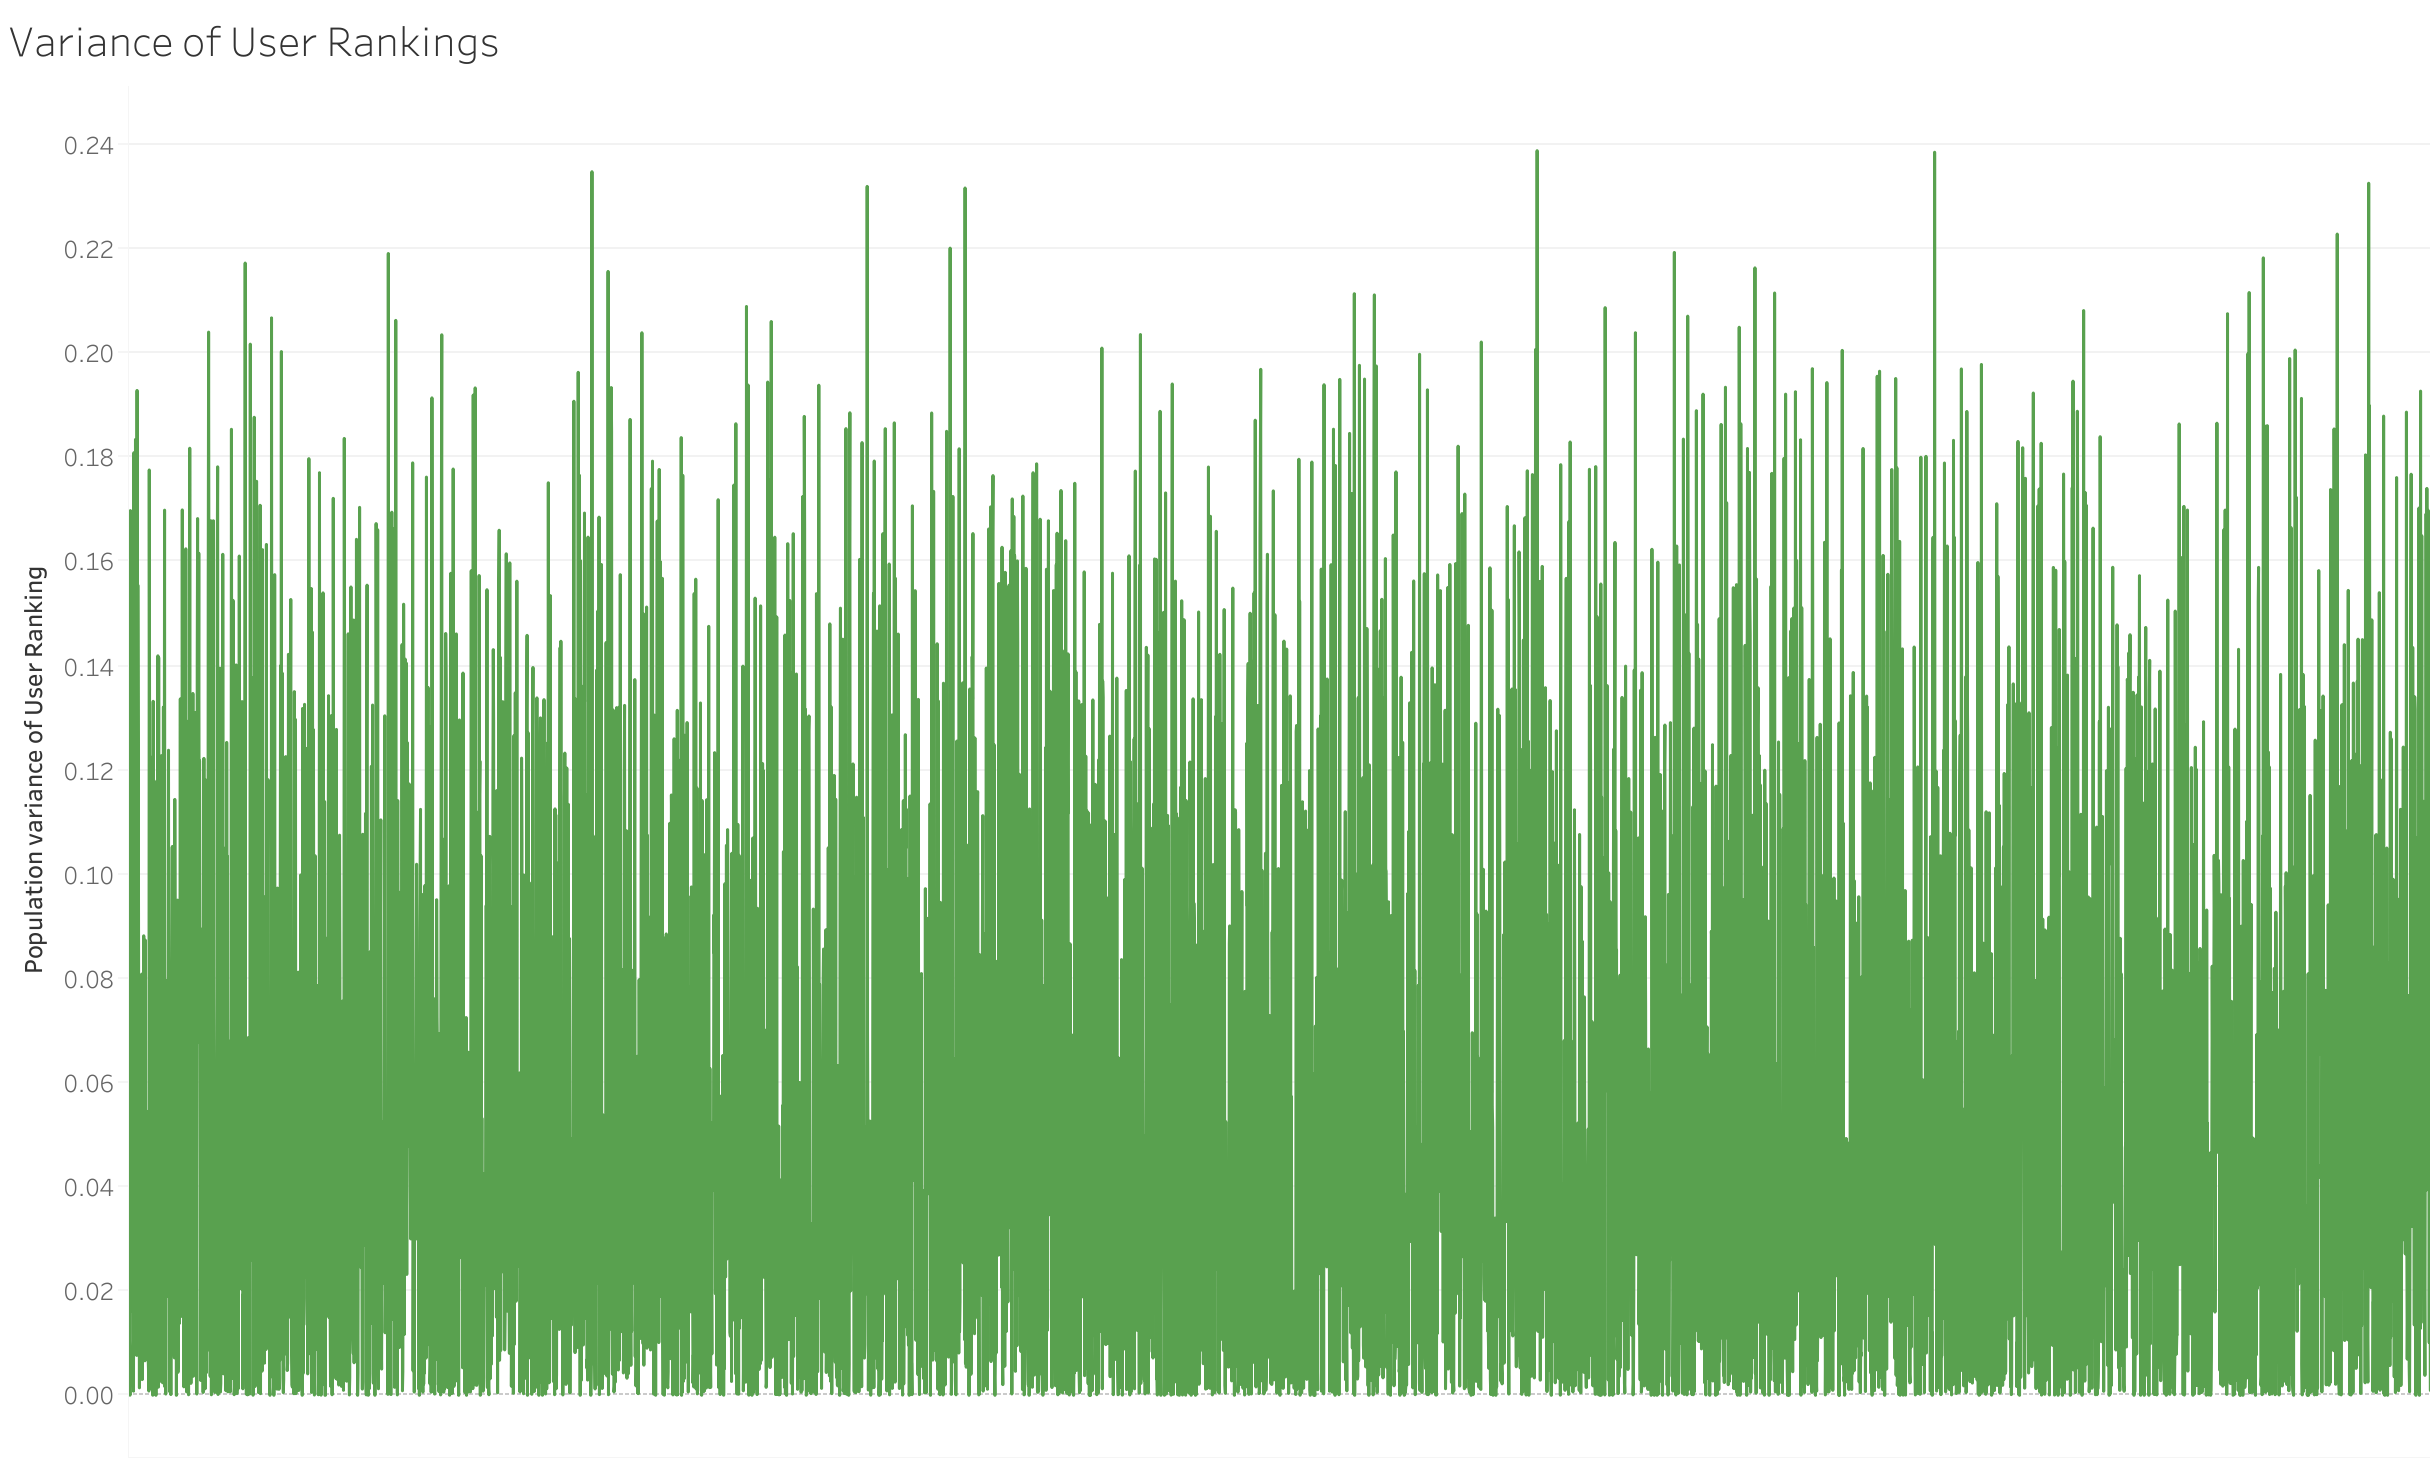
\includegraphics[scale=0.20]{images/VarianceofUserRankings.png}
\caption{Variance of User Rankings}
\label{image:variance_of_user_rankings}
\end{figure}

Our third and final finding defends our third claim that the execution time will be comparable to both the previous prediction-based and \gls{2pl} schedulers. When comparing all of the schedulers execution time over different workloads (see Figure \ref{image:scheduler_comparison}) we can see the differing execution times however, even with the differing execution times the overhead of the dynamic reputation system is comparable and a feasible solution. This defends our third and final claim that the dynamic reputation solution is a feasible solution but as we examine the data we can be more precise of when the solution should be legitimately considered.

After examining the data we see that the execution time is directly related to the workload. The defining difference of the workloads is the percentage of conflicting transactions in the workload. As the percentage of conflict increases in the differing workloads you can see the schedulers begin to execute at different execution times. 

From the graph in Figure \ref{image:scheduler_comparison} we can deduce that the best environment for the dynamic reputation solution is within execution environments that contain greater than 20\% conflicting transactions. Execution environments with high levels of conflict can benefit from the dynamic reputation solution while environments with less than 20\% conflict would be impacted by the overhead of processing within the dynamic reputation solution.

\begin{figure}
\centering
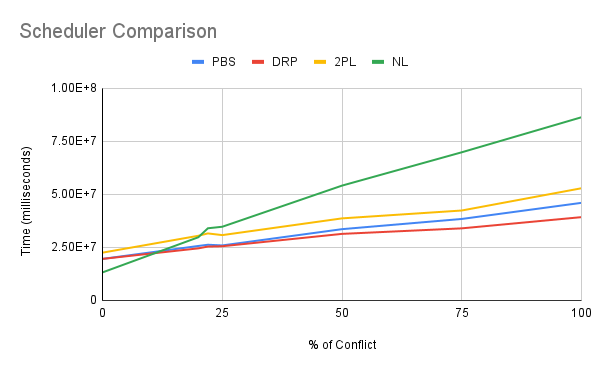
\includegraphics[scale=0.60]{images/SchedulerComparison.png}
\caption{Scheduler Comparison}
\label{image:scheduler_comparison}
\end{figure}

With our findings defending all three of our claims we can with confidence claim that the dynamic reputation solution provides a low overhead resource management solution with consistent scheduling.
